\section{Queueing Processes as Regulated Random Walks}
\label{sec:queu-proc-as}

\subsection*{Theory and Exercises}

\Opensolutionfile{hint}
\Opensolutionfile{ans}



In the construction of queueing processes as set out in
Section~\ref{sec:constr-discr-time} we are given two sequences of
i.i.d. random variables: the number of arrivals $\{a_k\}$ per period
and the service capacities $\{c_k\}$. Assuming that jobs can be served
in the period they arrive, the departure and queue length processes
are generated by the recursions
\begin{equation}\label{eq:5}
  \begin{split}
  Q_k &= [Q_{k-1}+a_k - c_k]^+,\\
  d_k &= Q_{k-1} +a_k- Q_{k},
  \end{split}
\end{equation}
where $[x]^+ := \max\{x, 0\}$.  

\begin{exercise}
  What is the difference between the recursive schemes of~(\ref{eq:5}) and~(\ref{eq:31})? Explain in the former scheme
  the formula for $d_k$.  
  \begin{hint}
When are the arrivals in slot $k$
    available for service in either of the systems?
  \end{hint}
\begin{solution}
  In the scheme
  \begin{equation*}
    \begin{split}
      d_k &= \min\{Q_{k-1}, c_k\}\\
Q_k &= Q_{k-1} + a_k - d_k,
    \end{split}
  \end{equation*}
the arrivals are assumed to arrive \emph{at the end} of period $k$. 

When we use the other scheme,
  \begin{equation*}
    \begin{split}
      Q_k &= [Q_{k-1} + a_k - c_k]^+,\\
      d_k &= Q_{k-1} + a_k - Q_k,
    \end{split}
  \end{equation*}
  we assume that the arrivals are available at the start of the $k$th
  slot. Observe that the number of jobs that enter the $k$th slot is
  $Q_{k-1}+a_k$. The number that remain at the end is $Q_k$. Thus, the
  number of jobs that depart must be the difference between what
  enters and what is left behind.
\end{solution}
\end{exercise}


Observe now that the relation for $Q_k$ shares a resemblance to a random walk $\{Z_k, k=0,1,\ldots\}$ with  $Z_k$ given by
\begin{equation}\label{eq:44}
  Z_k = Z_{k-1} + a_k - c_k.
\end{equation}
To see that $\{Z_k\}$ is indeed a random walk, observe that $Z$ makes  jumps of size $a_k-c_k, k=1,\ldots$, and $\{a_k-c_k\}$ is a sequence of i.i.d. random variables since, by assumption,  $\{a_k\}$ and $\{c_k\}$ are i.i.d.

Clearly, $\{Z_k\}$ is `free', i.e., it can take positive and negative
values, but $\{Q_k\}$ is restricted to the non-negative integers.  In
this section we show how to build the queueing process $\{Q_k\}$ from
the random walk $\{Z_k\}$ by a device called a \emph{reflection map}, which gives an  elegant construction of a queueing process. Moreover, we can use the probabilistic
tools that have been developed for the random walk to analyze queueing
systems. One example is the distribution of the time until an
especially large queue length is reached; these times can be
formulated as \emph{hitting times} of the random walk. Another example
is the average time it takes to clear a large queue.

\begin{exercise}
Show that  $Q_k$ satisfies the relation
\begin{equation}\label{eq:reich1}
  Q_k = Z_k - \min_{0\leq i \leq k} Z_i\wedge 0,
\end{equation}
where $Z_k$ is defined by the above random walk and
we write $a\wedge b$ for $\min\{a,b\}$.
\begin{hint}
Note first that from the expression for $Z_k$,
  $a_k - c_k = Z_k - Z_{k-1}$. Use this to get
  $Q_k = [Q_{k-1} +Z_k- Z_{k-1}]^+$. Subtract $Z_k$ from both sides, use recursion and
  use subsequently,
\begin{align*}
&\max\{\max\{a,b\}, c\} = \max\{a,b,c\}, \\
&Q_0 = Z_0, \\
&\max\{-a, -b \} = -\min\{a,b\}.
\end{align*}
\end{hint}
\begin{solution}
Note first that from the expression
for $Z_k$, $a_k - c_k = Z_k - Z_{k-1}$. Using this in the recursion
for $Q_k$, we get
\begin{equation*}
  Q_k = [Q_{k-1} +Z_k- Z_{k-1}]^+,
\end{equation*}
thus, 
\begin{equation*}
  Q_k - Z_{k} = \max\{Q_{k-1} - Z_{k-1}, -Z_k\}.
\end{equation*}
From this, using recursion and the hints, we see that
\begin{equation*}
  \begin{split}
  Q_k - Z_{k} 
% &= \max\{Q_{k-1} - Z_{k-1}, -Z_k\} \\
&= \max\{\max\{Q_{k-2} - Z_{k-2}, -Z_{k-1}\}, -Z_k\} \\
&= \max\{Q_{k-2} - Z_{k-2}, -Z_{k-1}, -Z_k\} \\
&= \max\{Q_{0} - Z_{0}, -Z_1, \ldots, -Z_k\} \\
&= \max\{0, -Z_1, \ldots, -Z_k\} \\
&= - \min\{0, Z_1, \ldots, Z_k\}.
  \end{split}
  \end{equation*}
For further discussion, if you are interested, refer to
  \citet{baccelli88:_sampl_m_m}.
\end{solution}
\end{exercise}

This recursion for $Q_k$ leads to really interesting graphs. In Figure~\ref{fig:random_bernoulli}
 we take $a_k \sim B(0.3)$, i.e., $a_k$ is Bernoulli-distributed with success
parameter $p=0.3$, i.e., $\P{a_k = 1} = 0.3 = 1- \P{a_k=0}$, and
$c_k \sim B(0.4)$. In Figure~\ref{fig:random_walk},  $a_k\sim B(0.49)$ and
the random walk is constructed as
\begin{equation}\label{eq:51}
  Z_k = Z_{k-1} + 2 a_k -1.
\end{equation}
Thus, if $a_k=1$, the random walk increases by one step, while if $a_k=0$, the random walk decreases by one step, so that $Z_k \neq Z_{k-1}$  always. Observe that this is slightly different from a random walk that satisfies~\eqref{eq:44}; there, $Z_{k}=Z_{k-1}$, if $a_k=c_k$.


\begin{figure}[ht]
  \centering
% see progs/reflected_random_walk.py
% This file was created by matplotlib2tikz v0.5.15.
\begin{tikzpicture}

\definecolor{color0}{rgb}{0.886274509803922,0.290196078431373,0.2}
\definecolor{color1}{rgb}{0.203921568627451,0.541176470588235,0.741176470588235}
\definecolor{color2}{rgb}{0.596078431372549,0.556862745098039,0.835294117647059}

\begin{groupplot}[group style={group size=1 by 2}]
\nextgroupplot[
title={Regulated Bernoulli Walk},
ylabel={Arrivals/services},
xmin=0, xmax=30,
ymin=-5, ymax=2,
width=12cm,
height=5cm,
tick align=outside,
xmajorgrids,
x grid style={white},
ymajorgrids,
y grid style={white},
axis line style={white},
axis background/.style={fill=white!89.803921568627459!black},
legend style={at={(0.03,0.03)}, anchor=south west, draw=white, fill=white!89.803921568627459!black},
legend entries={{A},{S},{Z}},
legend cell align={left}
]
\addplot [color0, mark=triangle*, mark size=2, mark options={solid}, only marks]
table {%
0 0
1 0
2 1
3 1
4 0
5 0
6 0
7 0
8 0
9 0
10 0
11 0
12 0
13 0
14 0
15 1
16 0
17 0
18 0
19 0
20 0
21 0
22 0
23 0
24 0
25 0
26 1
27 1
28 0
29 0
};
\addplot [color1, mark=triangle*, mark size=2, mark options={solid,rotate=180}, only marks]
table {%
0 0
1 -1
2 0
3 0
4 0
5 0
6 0
7 0
8 -1
9 0
10 -1
11 -1
12 -1
13 0
14 0
15 0
16 0
17 0
18 0
19 0
20 0
21 0
22 0
23 -1
24 -1
25 0
26 -1
27 0
28 -1
29 -1
};
\addplot [color2, mark=*, mark size=1, mark options={solid,draw=black}]
table {%
0 0
1 -1
2 0
3 1
4 1
5 1
6 1
7 1
8 0
9 0
10 -1
11 -2
12 -3
13 -3
14 -3
15 -2
16 -2
17 -2
18 -2
19 -2
20 -2
21 -2
22 -2
23 -3
24 -4
25 -4
26 -4
27 -3
28 -4
29 -5
};
\nextgroupplot[
ylabel={Queue},
xmin=0, xmax=30,
ymin=-5, ymax=2,
width=12cm,
height=5cm,
tick align=outside,
xmajorgrids,
x grid style={white},
ymajorgrids,
y grid style={white},
axis line style={white},
axis background/.style={fill=white!89.803921568627459!black},
legend style={at={(0.03,0.03)}, anchor=south west, draw=white, fill=white!89.803921568627459!black},
legend entries={{Z},{Q}},
legend cell align={left}
]
\addplot [color0, mark=*, mark size=1, mark options={solid,draw=black}]
table {%
0 0
1 -1
2 0
3 1
4 1
5 1
6 1
7 1
8 0
9 0
10 -1
11 -2
12 -3
13 -3
14 -3
15 -2
16 -2
17 -2
18 -2
19 -2
20 -2
21 -2
22 -2
23 -3
24 -4
25 -4
26 -4
27 -3
28 -4
29 -5
};
\addplot [color1, mark=*, mark size=2, mark options={solid,draw=black}]
table {%
0 0
1 0
2 1
3 2
4 2
5 2
6 2
7 2
8 1
9 1
10 0
11 0
12 0
13 0
14 0
15 1
16 1
17 1
18 1
19 1
20 1
21 1
22 1
23 0
24 0
25 0
26 0
27 1
28 0
29 0
};
\end{groupplot}

\end{tikzpicture}
%% This file was created by matplotlib2tikz v0.5.15.
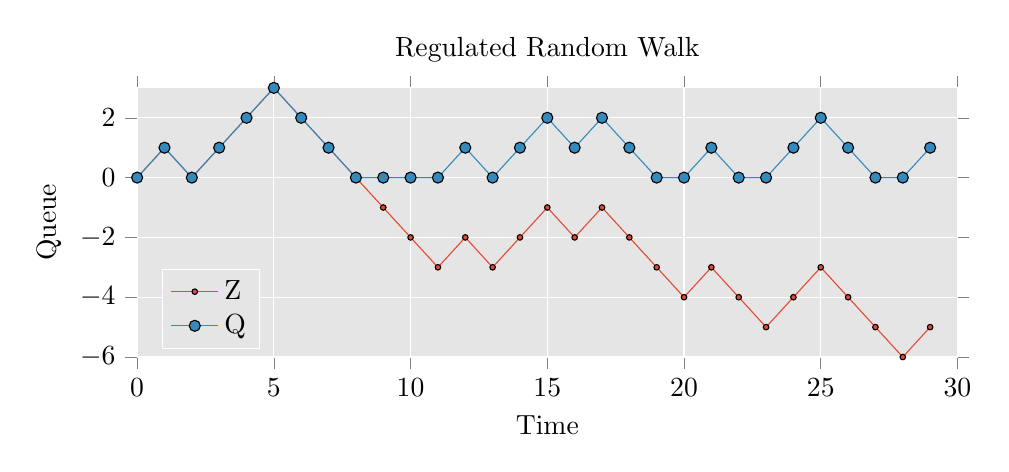
\begin{tikzpicture}

\definecolor{color0}{rgb}{0.886274509803922,0.290196078431373,0.2}
\definecolor{color1}{rgb}{0.203921568627451,0.541176470588235,0.741176470588235}

\begin{axis}[
title={Regulated Random Walk},
xlabel={Time},
ylabel={Queue},
xmin=0, xmax=30,
ymin=-6, ymax=3,
width=12cm,
height=5cm,
tick align=outside,
xmajorgrids,
x grid style={white},
ymajorgrids,
y grid style={white},
axis line style={white},
axis background/.style={fill=white!89.803921568627459!black},
legend style={at={(0.03,0.03)}, anchor=south west, draw=white, fill=white!89.803921568627459!black},
legend entries={{Z},{Q}},
legend cell align={left}
]
\addplot [color0, mark=*, mark size=1, mark options={solid,draw=black}]
table {%
0 0
1 1
2 0
3 1
4 2
5 3
6 2
7 1
8 0
9 -1
10 -2
11 -3
12 -2
13 -3
14 -2
15 -1
16 -2
17 -1
18 -2
19 -3
20 -4
21 -3
22 -4
23 -5
24 -4
25 -3
26 -4
27 -5
28 -6
29 -5
};
\addplot [color1, mark=*, mark size=2, mark options={solid,draw=black}]
table {%
0 0
1 1
2 0
3 1
4 2
5 3
6 2
7 1
8 0
9 0
10 0
11 0
12 1
13 0
14 1
15 2
16 1
17 2
18 1
19 0
20 0
21 1
22 0
23 0
24 1
25 2
26 1
27 0
28 0
29 1
};
\end{axis}

\end{tikzpicture}
\caption{The upper panel shows a graph of the random walk $Z$. An
  upward pointing triangle corresponds to an arrival, a downward
  triangle to a potential service. The lower panel shows the queueing
  process $\{Q_k\}$ as a random walk with reflection.}
\label{fig:random_bernoulli}
\end{figure}

\begin{figure}[ht]
  \centering
% see progs/reflected_random_walk.py
% This file was created by matplotlib2tikz v0.5.15.
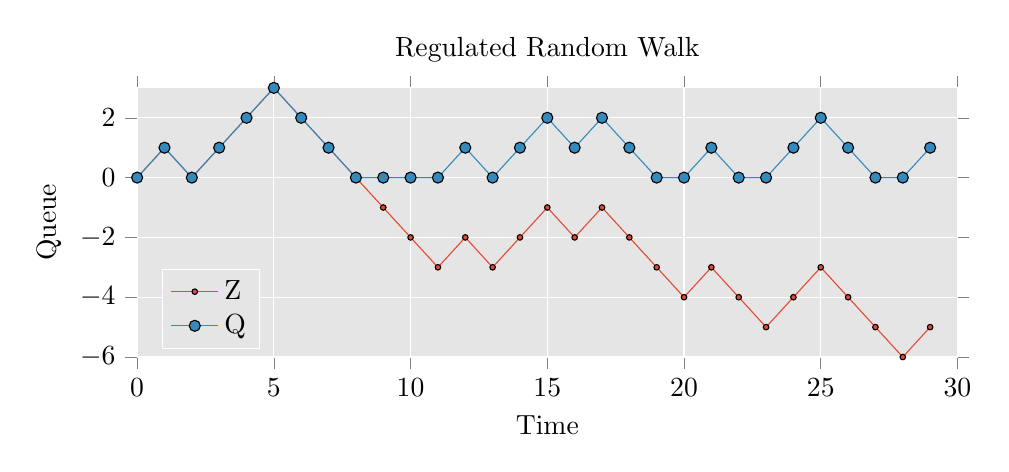
\begin{tikzpicture}

\definecolor{color0}{rgb}{0.886274509803922,0.290196078431373,0.2}
\definecolor{color1}{rgb}{0.203921568627451,0.541176470588235,0.741176470588235}

\begin{axis}[
title={Regulated Random Walk},
xlabel={Time},
ylabel={Queue},
xmin=0, xmax=30,
ymin=-6, ymax=3,
width=12cm,
height=5cm,
tick align=outside,
xmajorgrids,
x grid style={white},
ymajorgrids,
y grid style={white},
axis line style={white},
axis background/.style={fill=white!89.803921568627459!black},
legend style={at={(0.03,0.03)}, anchor=south west, draw=white, fill=white!89.803921568627459!black},
legend entries={{Z},{Q}},
legend cell align={left}
]
\addplot [color0, mark=*, mark size=1, mark options={solid,draw=black}]
table {%
0 0
1 1
2 0
3 1
4 2
5 3
6 2
7 1
8 0
9 -1
10 -2
11 -3
12 -2
13 -3
14 -2
15 -1
16 -2
17 -1
18 -2
19 -3
20 -4
21 -3
22 -4
23 -5
24 -4
25 -3
26 -4
27 -5
28 -6
29 -5
};
\addplot [color1, mark=*, mark size=2, mark options={solid,draw=black}]
table {%
0 0
1 1
2 0
3 1
4 2
5 3
6 2
7 1
8 0
9 0
10 0
11 0
12 1
13 0
14 1
15 2
16 1
17 2
18 1
19 0
20 0
21 1
22 0
23 0
24 1
25 2
26 1
27 0
28 0
29 1
};
\end{axis}

\end{tikzpicture}
\caption{Another example of a reflected random walk.}
\label{fig:random_walk}
\end{figure}


With~(\ref{eq:reich1}),  we see that a random walk $\{Z_k\}$ can be converted into a queueing
process $\{Q_k\}$, and we might try to understand the transient behavior of the latter by investigating the transient behavior of the former.  For this, we first relate the random walk of the type~\eqref{eq:51} to a random walk in continuous time. 

\begin{exercise}
  Let $N_{\lambda+\mu}$ be a Poisson process with rate $\lambda+\mu$. If $\{a_k\}$ is an i.i.d. sequence of Bernoulli random variables such that $\P{a_k=1} = \lambda/(\lambda+\mu)=1-\P{a_k=0}$, show that the random variable
  \begin{equation*}
    N_\lambda(t) = \sum_{k=1}^\infty a_k \1{k \leq N_{\lambda+\mu}(t)},
  \end{equation*}
has a Poisson distribution with rate $\lambda t$. 
\begin{solution}
  From Exercise~\ref{ex:1} we know that thinning  a rate $\lambda$ Poisson process  with i.i.d. Bernoulli random variables with success probability $p$  leads to another Poisson process with rate $\lambda p$. In the present case, the original Poisson process has rate $\lambda+\mu$ and $p=\lambda/(\lambda+\mu)$. Hence, the random variable $N_{\lambda t}\sim P\left(\frac\lambda{\lambda+\mu} (\lambda+\mu)t\right) = P(\lambda t)$.
\end{solution}
\end{exercise}

Similarly, let
\begin{equation*}
  N_\mu(t) = N_{\lambda+\mu}(t) - N_\lambda(t) = \sum_{k=1}^\infty (1-a_k) \1{N_{\lambda+\mu}(t) \leq k};
\end{equation*}
but this is $N_{\lambda+\mu}(t)$ thinned by the Bernoulli random variables $\{1-a_k\}$. Let  $N_\lambda = \{N_\lambda(t)\}$ and $N_\mu = \{N_\mu(t)\}$  be the associated Poisson processes. 

With the processes $N_\lambda$ and $N_\mu$ constructed above from the sequence $\{a_k\}$ and the Poisson process $N_{\lambda+\mu}$ we can define the process $Z=\{Z(t)\}$ such that
\begin{equation*}
  Z(t) = Z(0)+N_\lambda(t) - N_\mu(t).
\end{equation*}
Thus, we let $N_\lambda$ correspond to job  arrivals and $N_\mu$ to departures. Observe that the times $\{T_k\}$ at which $Z$ makes jumps are such that $T_k-T_{k-1}$ have exponential distribution with mean $1/(\lambda+\mu)$. At the jump times, $Z(T_k) = Z_k$, where $Z_k$ satisfies~\eqref{eq:51} with $\P{a_k = 1} = \lambda/(\lambda+\mu)$.  We call $Z$ the \emph{free} $M/M/1$ queue as, contrary to the real $M/M/1$ queue, $Z$ can take negative values. 

\begin{exercise}  
Show that
\begin{equation*}
    \P{Z(t)=n}_m 
= e^{-(\lambda+\mu)t} \left(\frac\lambda\mu\right)^{(n-m)/2} \sum_{k=0}^\infty 
\frac{(t\sqrt{\lambda\mu} )^{2k+m-n}}{k!(k+m-n)!},
\end{equation*}
where $\P{\cdot}_m$ means that the random walk starts at $m$, i.e.,
$Z(0)=m$.

As an aside, the summation includes negative factorials when
$k+m-n<0$. The tacit assumption is to take $n!\in \{\pm \infty\}$ for
$n\in \Z_-$. Another way to get around this problem is to take
$k=\max\{0, m-n\}$..
\begin{hint}
It is actually not hard, even though the expression looks
  hard. Use conditioning to see that
  $\P{Z(t)=n}_m = \P{N_\mu(t) - N_\lambda(t) = m - n}$. Then write out
  the definitions of the two Poisson distributions. Assemble
  terms. Then fiddle a bit with the terms to get~$t\sqrt{\lambda\mu}$. 
\end{hint}
\begin{solution}
With this we have a characterization of the queue length process as a
function of time until it hits zero for the first time. What can we
say about the distribution of $Q(t)$? With the above random walk, 
\begin{equation}\label{eq:29}
  \begin{split}
    \P{Z(t)=n}_m
&= \P{m+N_\lambda(t) - N_\mu(t) = n }  = \P{N_\lambda(t) - N_\mu(t) = n-m }  \\
&= \P{N_\mu(t) - N_\lambda(t) = m-n }  \\
&= \sum_{k=0}^\infty \P{N_\mu(t) = k - n + m\given N_\lambda(t) = k } \P{N_\lambda(t)=k}\\
&= \sum_{k=0}^\infty e^{-\mu t} \frac{(\mu t)^{k -n+m}}{(k-n +m)!} e^{-\lambda t} \frac{(\lambda t)^k}{k!} \\
&= e^{-(\lambda+\mu)t} \sum_{k=0}^\infty \frac{(\lambda t)^k(\mu t)^{k  -n + m }}{k!(k-n+m)!}.
  \end{split}
\end{equation}
We can write this a bit simpler by noting that
\begin{equation*}
  \begin{split}
  (\lambda t)^k (\mu t) ^{k + m - n}  
&=  \lambda^k t^k\mu^{k + m - n} t^{k+m-n} \\
&= \lambda^k \mu^{k + m - n} (t\sqrt{\lambda \mu})^{2k+m-n} (\lambda\mu)^{-k + (n-m)/2} \\
&= (\lambda/\mu)^{(n-m)/2} (t\sqrt{\lambda \mu})^{2k+m-n}.
  \end{split}
\end{equation*}
With this,
\begin{equation*}
    \P{Z(t)=n} 
= e^{-(\lambda+\mu)t} \left(\frac\lambda\mu\right)^{(n-m)/2} \sum_{k=0}^\infty 
\frac{(t\sqrt{\lambda\mu} )^{2k+m-n}}{k!(k+m-n)!}.
\end{equation*}
\end{solution}
\end{exercise}


The solution of the above exercise shows that there is no simple
function by which we can compute the transient distribution of 
this simple random walk $Z$. Since a queueing process is typically a
more complicated object (as we need to obtain $Q$ from $Z$ via~\eqref{eq:reich1}), our
hopes to finding anything simple for the transient analysis of the
$M/M/1$ queue should not be too high. And the $M/M/1$ is but the
simplest queueing system; other queueing systems will be more
complicated yet.  We therefore give up the analysis of such transient
queueing systems and we henceforth contend ourselves with the analysis
of queueing systems in the limit as $t\to\infty$.  This of course
warrants two questions: what type of limit is actually meant here, and
what is the rate of convergence to this limiting situation? We address
these questions subsequently.

The \emph{long-run limiting behavior} of a queueing system (i.e., the first question) is an
important topic by itself. The underlying question is what happens if
we simulate the system for a long time. For instance, does there exist
a random variable $Q$ such that $Q_k\to Q$ in some sense? The answer
to this question is in the affirmative, provided some simple stability
conditions are satisfied, see
Section~\ref{sec:rate-stability}. However, it requires a considerable
amount of mathematics to make this procedure precise. To sketch what
has to be done, first, we need to define $\{Q_k\}$ as random variables
in their own right. Note that up to now we just considered each $Q_k$
as a \emph{number}, i.e., a measurement or simulation of the queue
length time of the $k$th period. Defining $Q_k$ as a random variable
is not as simple as the definition of, for instance, the number of
arrivals $\{a_k\}$; these random variables can be safely
\emph{assumed} to be i.i.d. However, the queue lengths $\{Q_k\}$ are
certainly not i.i.d., but, as should be apparent from
Eq.~\eqref{eq:59}, they are \emph{constructed} in terms of
recursions. Next, based on these recursions, we need to show that the
sequence of distribution functions $\{G_k\}$ associated with the
random variables $\{Q_k\}$ converges to some limiting distribution
function~$G$, say. Finally, it is necessary to show that it is
possible to construct a random variable~$Q$ that has~$G$ as its
distribution function.  In this sense, then, we can say
that~$Q_k \to Q$. The random variable $Q$ is known as the
\recall{steady-state limit} of the sequence of random variables
$\{Q_k\}$, and the distribution $G$ of~$Q$ is known as the
\recall{limiting} or \emph{stationary distribution} of $\{Q_k\}$.

In these notes we sidestep all these fundamental issues, as the
details require measure theory and more advanced probability theory
than we can deal with in this course. However, it can all be made
precise. 

We illustrate the rate of convergence to the limiting situation (i.e., the second question) by means of an example. Specifically, we consider the sequence of waiting times $\{W_{Q,k}\}$ to a limiting random variable $W_Q$, where $W_{Q,k}$ is constructed according to the recursion
Eq.~(\ref{eq:56}). Suppose that $X_k\sim U\{1,2,4\}$ and
$S_k\sim U\{1,2,3\}$.  Starting with $W_{Q,0}=5$ we use
Eq.~(\ref{eq:56}) to compute the \emph{exact} distribution of
$W_{Q,k}$ for $k=1,2,\ldots, 20$, c.f., the left panel in
Figure~\ref{fig:convergence}. We see that when $k=5$, the `hump' of
$\P{W_{Q,5}=x}$ around $x=5$ is due the starting value of
$W_{Q,0}=5$. However, for $k>10$ the distribution of $W_{Q,k}$ hardly
changes, at least not visually. Apparently, the convergence of the
sequence of distributions of $W_{Q,k}$ is rather fast. In the middle
panel we show the results of a set of \emph{simulations} for
increasing simulation length, up to $N=1000$ samples. Here the
\emph{empirical distribution} for the simulation is defined as
\begin{equation*}
\P{W_Q\leq x} =   \frac 1n \sum_{k=1}^n \1{W_{Q,k} \leq x},
\end{equation*}
where $W_{Q,k}$ is obtained by simulation. As should be clear from the
figure, the simulated distribution also seems to converge quite fast to
some limiting function. Finally, in the right hand panel we compare
the densities as obtained by the exact method and simulation with
$n=1000$. Clearly, for all practical purposes, these densities can be
treated as the same.

The combination of the fast convergence to the steady-state situation
and the difficulties with the transient analysis validates, to some
extent, that most queueing theory is concerned with the analysis of
the system in \emph{stationarity}. The study of queueing systems in
stationary state will occupy us for the rest of the book.

\begin{figure}
  \centering
% see progs/waiting_time_simulation.py
% This file was created by matplotlib2tikz v0.6.18.
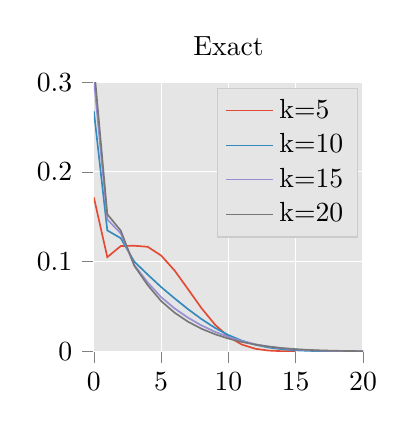
\begin{tikzpicture}

\definecolor{color0}{rgb}{0.886274509803922,0.290196078431373,0.2}
\definecolor{color1}{rgb}{0.203921568627451,0.541176470588235,0.741176470588235}
\definecolor{color2}{rgb}{0.596078431372549,0.556862745098039,0.835294117647059}

\begin{axis}[
axis background/.style={fill=white!89.80392156862746!black},
axis line style={white},
height=5cm,
legend cell align={left},
legend entries={{k=5},{k=10},{k=15},{k=20}},
legend style={draw=white!80.0!black, fill=white!89.80392156862746!black},
tick align=outside,
tick pos=left,
title={Exact},
width=5cm,
x grid style={white},
xmajorgrids,
xmin=0, xmax=20,
y grid style={white},
ymajorgrids,
ymin=0, ymax=0.3
]
\addlegendimage{no markers, color0}
\addlegendimage{no markers, color1}
\addlegendimage{no markers, color2}
\addlegendimage{no markers, white!46.666666666666664!black}
\addplot [semithick, color0]
table [row sep=\\]{%
0	0.171637114938441 \\
1	0.104963674236651 \\
2	0.117394028688039 \\
3	0.117715795356399 \\
4	0.116547274297617 \\
5	0.10680959880777 \\
6	0.0901116022286576 \\
7	0.0692645091364799 \\
8	0.048095649375942 \\
9	0.0298057545428373 \\
10	0.0162068790326678 \\
11	0.00753611407475148 \\
12	0.00287896492743315 \\
13	0.000846754390421514 \\
14	0.000169350878084303 \\
15	1.69350878084303e-05 \\
};
\addplot [semithick, color1]
table [row sep=\\]{%
0	0.267670098481664 \\
1	0.134811729932366 \\
2	0.126115559618164 \\
3	0.100031570893792 \\
4	0.0856111019982735 \\
5	0.0716606125484384 \\
6	0.0590583363688737 \\
7	0.0470211200764174 \\
8	0.0359432992083069 \\
9	0.0262065053330494 \\
10	0.0181445546165273 \\
11	0.0118798282991401 \\
12	0.0073250777973754 \\
13	0.00423423971833927 \\
14	0.00228253344190638 \\
15	0.0011402678063088 \\
16	0.000523855446719374 \\
17	0.000219223477018188 \\
18	8.25631776709328e-05 \\
19	2.75497389435522e-05 \\
20	7.97697729519009e-06 \\
21	1.94735298174807e-06 \\
22	3.84308246766187e-07 \\
23	5.73594398158488e-08 \\
24	5.73594398158488e-09 \\
25	2.86797199079244e-10 \\
};
\addplot [semithick, color2]
table [row sep=\\]{%
0	0.30317953657453 \\
1	0.14699251783874 \\
2	0.131469895956502 \\
3	0.0963326761914749 \\
4	0.076869973873194 \\
5	0.0604280411223663 \\
6	0.04784522712146 \\
7	0.0374709958541702 \\
8	0.0289083894170772 \\
9	0.0218171288010453 \\
10	0.0160366591920489 \\
11	0.0114368309310598 \\
12	0.00789001335365536 \\
13	0.00525183269083643 \\
14	0.00336515460534012 \\
15	0.0020710966262499 \\
16	0.00122159902225598 \\
17	0.00068892069543721 \\
18	0.000370520942164379 \\
19	0.000189507686033138 \\
20	9.18799257332931e-05 \\
21	4.20732116476868e-05 \\
22	1.8119623555642e-05 \\
23	7.30325357242076e-06 \\
24	2.73902579612197e-06 \\
25	9.49296970741557e-07 \\
26	3.01535089774823e-07 \\
27	8.68973074166946e-08 \\
28	2.24352547533544e-08 \\
29	5.10658224714927e-09 \\
30	1.00330207473452e-09 \\
31	1.65305808238278e-10 \\
32	2.1904780230781e-11 \\
33	2.18562108732849e-12 \\
34	1.45708072488566e-13 \\
35	4.85693574961886e-15 \\
};
\addplot [semithick, white!46.666666666666664!black]
table [row sep=\\]{%
0	0.319144828865997 \\
1	0.152832481719423 \\
2	0.134555843047554 \\
3	0.0955843772093346 \\
4	0.0738400658782454 \\
5	0.0560416473000174 \\
6	0.0430735344931855 \\
7	0.0330094400597946 \\
8	0.0252025073900232 \\
9	0.0190619218519665 \\
10	0.0142314981096182 \\
11	0.0104502968908312 \\
12	0.00752571097051776 \\
13	0.00530189974927228 \\
14	0.0036465388505557 \\
15	0.00244409730130202 \\
16	0.00159388825481048 \\
17	0.00100987966393171 \\
18	0.000620806320781876 \\
19	0.000369768373140325 \\
20	0.000213105770501226 \\
21	0.000118668173969863 \\
22	6.37517889450218e-05 \\
23	3.29887723679431e-05 \\
24	1.64131133653723e-05 \\
25	7.83660826357756e-06 \\
26	3.58303411938414e-06 \\
27	1.56505220483645e-06 \\
28	6.51341807039512e-07 \\
29	2.57510039633041e-07 \\
30	9.63864754135865e-08 \\
31	3.40252853261261e-08 \\
32	1.12779804213856e-08 \\
33	3.49207550281559e-09 \\
34	1.00407169477642e-09 \\
35	2.66202450453925e-10 \\
36	6.45301076626973e-11 \\
37	1.41567960213762e-11 \\
38	2.77528281343393e-12 \\
39	4.78404346590005e-13 \\
40	7.10027762243559e-14 \\
41	8.8158372477798e-15 \\
42	8.78458124708791e-16 \\
43	6.58021067197597e-17 \\
44	3.29010533598798e-18 \\
45	8.22526333996996e-20 \\
};
\end{axis}

\end{tikzpicture}
% This file was created by matplotlib2tikz v0.6.18.
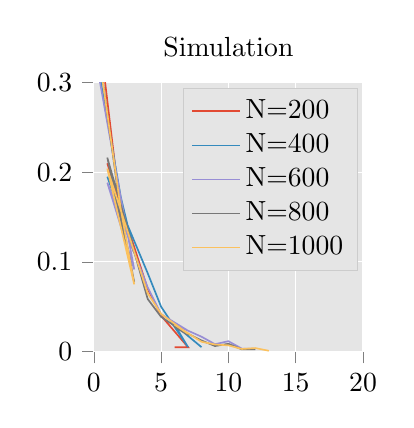
\begin{tikzpicture}

\definecolor{color0}{rgb}{0.886274509803922,0.290196078431373,0.2}
\definecolor{color1}{rgb}{0.203921568627451,0.541176470588235,0.741176470588235}
\definecolor{color2}{rgb}{0.596078431372549,0.556862745098039,0.835294117647059}
\definecolor{color3}{rgb}{0.984313725490196,0.756862745098039,0.368627450980392}

\begin{axis}[
axis background/.style={fill=white!89.80392156862746!black},
axis line style={white},
height=5cm,
legend cell align={left},
legend entries={{N=200},{N=400},{N=600},{N=800},{N=1000}},
legend style={draw=white!80.0!black, fill=white!89.80392156862746!black},
tick align=outside,
tick pos=left,
title={Simulation},
width=5cm,
x grid style={white},
xmajorgrids,
xmin=0, xmax=20,
y grid style={white},
ymajorgrids,
ymin=0, ymax=0.3
]
\addlegendimage{no markers, color0}
\addlegendimage{no markers, color1}
\addlegendimage{no markers, color2}
\addlegendimage{no markers, white!46.666666666666664!black}
\addlegendimage{no markers, color3}
\addplot [semithick, color0]
table [row sep=\\]{%
0	0.405 \\
2	0.155 \\
3	0.11 \\
1	0.21 \\
4	0.07 \\
5	0.04 \\
7	0.005 \\
6	0.005 \\
};
\addplot [semithick, color1]
table [row sep=\\]{%
0	0.345 \\
2	0.1725 \\
3	0.11 \\
1	0.195 \\
4	0.0875 \\
5	0.05 \\
7	0.005 \\
6	0.03 \\
8	0.005 \\
};
\addplot [semithick, color2]
table [row sep=\\]{%
0	0.338333333333333 \\
2	0.171666666666667 \\
3	0.0916666666666667 \\
1	0.188333333333333 \\
4	0.0716666666666667 \\
5	0.0416666666666667 \\
7	0.0233333333333333 \\
6	0.03 \\
8	0.0166666666666667 \\
9	0.00833333333333333 \\
10	0.0116666666666667 \\
11	0.00333333333333333 \\
12	0.00333333333333333 \\
};
\addplot [semithick, white!46.666666666666664!black]
table [row sep=\\]{%
0	0.375 \\
2	0.155 \\
3	0.0775 \\
1	0.21625 \\
4	0.05875 \\
5	0.03875 \\
7	0.01875 \\
6	0.0275 \\
8	0.0125 \\
9	0.00625 \\
10	0.00875 \\
11	0.0025 \\
12	0.0025 \\
};
\addplot [semithick, color3]
table [row sep=\\]{%
0	0.371 \\
2	0.159 \\
3	0.075 \\
1	0.204 \\
4	0.065 \\
5	0.042 \\
7	0.02 \\
6	0.03 \\
8	0.011 \\
9	0.008 \\
10	0.007 \\
11	0.003 \\
12	0.004 \\
13	0.001 \\
};
\end{axis}

\end{tikzpicture}
% This file was created by matplotlib2tikz v0.6.18.
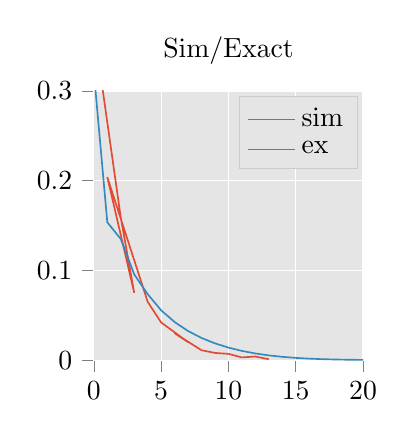
\begin{tikzpicture}

\definecolor{color0}{rgb}{0.886274509803922,0.290196078431373,0.2}
\definecolor{color1}{rgb}{0.203921568627451,0.541176470588235,0.741176470588235}

\begin{axis}[
axis background/.style={fill=white!89.80392156862746!black},
axis line style={white},
height=5cm,
legend cell align={left},
legend entries={{sim},{ex}},
legend style={draw=white!80.0!black, fill=white!89.80392156862746!black},
tick align=outside,
tick pos=left,
title={Sim/Exact},
width=5cm,
x grid style={white},
xmajorgrids,
xmin=0, xmax=20,
y grid style={white},
ymajorgrids,
ymin=0, ymax=0.3
]
\addlegendimage{no markers, color0}
\addlegendimage{no markers, color1}
\addplot [semithick, color0]
table [row sep=\\]{%
0	0.371 \\
2	0.159 \\
3	0.075 \\
1	0.204 \\
4	0.065 \\
5	0.042 \\
7	0.02 \\
6	0.03 \\
8	0.011 \\
9	0.008 \\
10	0.007 \\
11	0.003 \\
12	0.004 \\
13	0.001 \\
};
\addplot [semithick, color1]
table [row sep=\\]{%
0	0.321210551486458 \\
1	0.153610083372614 \\
2	0.134996882888543 \\
3	0.0955453595314327 \\
4	0.0735078887084144 \\
5	0.0555229800002277 \\
6	0.04248374875847 \\
7	0.0324340034608454 \\
8	0.0247003408996893 \\
9	0.0186641447360399 \\
10	0.0139463946460717 \\
11	0.0102694858215254 \\
12	0.00743088327585761 \\
13	0.00527073128751502 \\
14	0.00365717229905777 \\
15	0.00247795939414692 \\
16	0.00163698266495181 \\
17	0.00105290221377686 \\
18	0.000658507879443266 \\
19	0.000399962283965939 \\
20	0.000235625724146408 \\
21	0.000134469080633985 \\
22	7.42414402995369e-05 \\
23	3.9599462856611e-05 \\
24	2.03752070292254e-05 \\
25	1.00967419862763e-05 \\
26	4.81015048751568e-06 \\
27	2.19881789346049e-06 \\
28	9.62361553682428e-07 \\
29	4.0231467941736e-07 \\
30	1.60217273745469e-07 \\
31	6.05984076836477e-08 \\
32	2.1694159117719e-08 \\
33	7.32269701357755e-09 \\
34	2.32015184679573e-09 \\
35	6.86512898604053e-10 \\
36	1.88567121134715e-10 \\
37	4.77418033968616e-11 \\
38	1.10478769598855e-11 \\
39	2.31287446547169e-12 \\
40	4.32519221532182e-13 \\
41	7.10963979995277e-14 \\
42	1.0058482615638e-14 \\
43	1.19011335266025e-15 \\
44	1.12978561565232e-16 \\
45	8.06075807317056e-18 \\
46	3.83845622531931e-19 \\
47	9.13918148885551e-21 \\
};
\end{axis}

\end{tikzpicture}
%  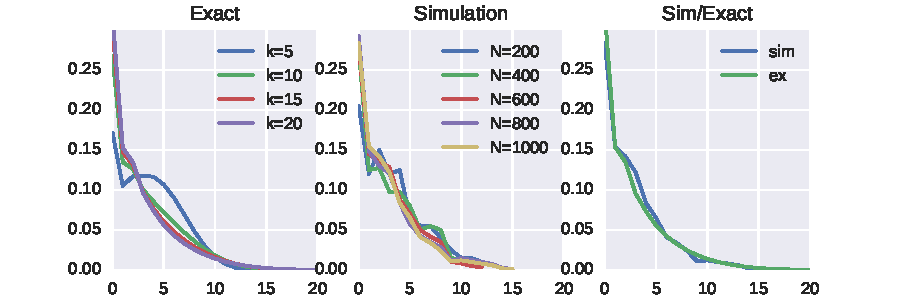
\includegraphics{progs/gg1convergence}
  \caption{The density of $W_{Q,k}$ for $k=5, 10, 15, 20$ computed by
    an exact method as compared the density obtained by simulation of
    different run lengths $N=200, 400, \ldots 1000$. The right panel
    compares the exact density of $W_{Q,20}$ to the density obtained by simulation
    for $N=1000$.}
\label{fig:convergence}
\end{figure}




\begin{exercise}
  Suppose that $X_k\in\{1,3\}$ such that $\P{X_k=1}=\P{X_k=3}$ and
  $S_k\in\{1,2\}$ with $\P{S_k=1}=\P{S_k=2}$. Write a computer program
  to see how fast the distributions of $W_{Q,k}$ converge to a limiting distribution function.
  \begin{solution}
Here is an example with python. In R it must be equally simple.
I compute the  difference, i.e., the Kolmogorov-Smirnov statistic, between
the distributions of $W_{Q,k-1}$ and $W_{Q,k}$, 
\begin{equation*}
  \max_x\{ |\P{W_{Q,k}\leq x} - \P{W_{Q,k-1}\leq x}|\},
\end{equation*}
for $x$ in the support of $W_{Q,k}$. 

\begin{pyconsole}
  
from lea import Lea

S = Lea.fromVals(1,  2)
X = Lea.fromVals(1,  3)
U = S-X

W = Lea.fromVals(3)
for k in range(1, 10):
    W_new = Lea.fastMax(W + U, 0)
    m = max(abs(W_new.cdf(x)-W.cdf(x))  for x in range(W_new.support()[-1]))
    print(k, m) 
    W = W_new

\end{pyconsole}

So, after some 10 customers, the distribution hardly changes anymore. 

  \end{solution}
  \end{exercise}

\begin{exercise}
  Validate the results of  Figure~\ref{fig:convergence} with simulation.
  \begin{solution}
    You can study \texttt{waiting\_time\_simulation.py} at
    \href{https://github.com/ndvanforeest/queueing_book/tree/master/progs}{github}
    if you like, but skipping it is OK. Trying to make the graph in
    your favorite programming language is fun.
\end{solution}
\end{exercise}

\Closesolutionfile{hint}
\Closesolutionfile{ans}

\opt{solutionfiles}{
\subsection*{Hints}
\input{hint}
\subsection*{Solutions}
\input{ans}
}
%\clearpage

%%% Local Variables:
%%% mode: latex
%%% TeX-master: "../book"
%%% End:
